\documentclass{standalone}
\usepackage{tikz}
\usetikzlibrary{patterns, positioning}

\begin{document}
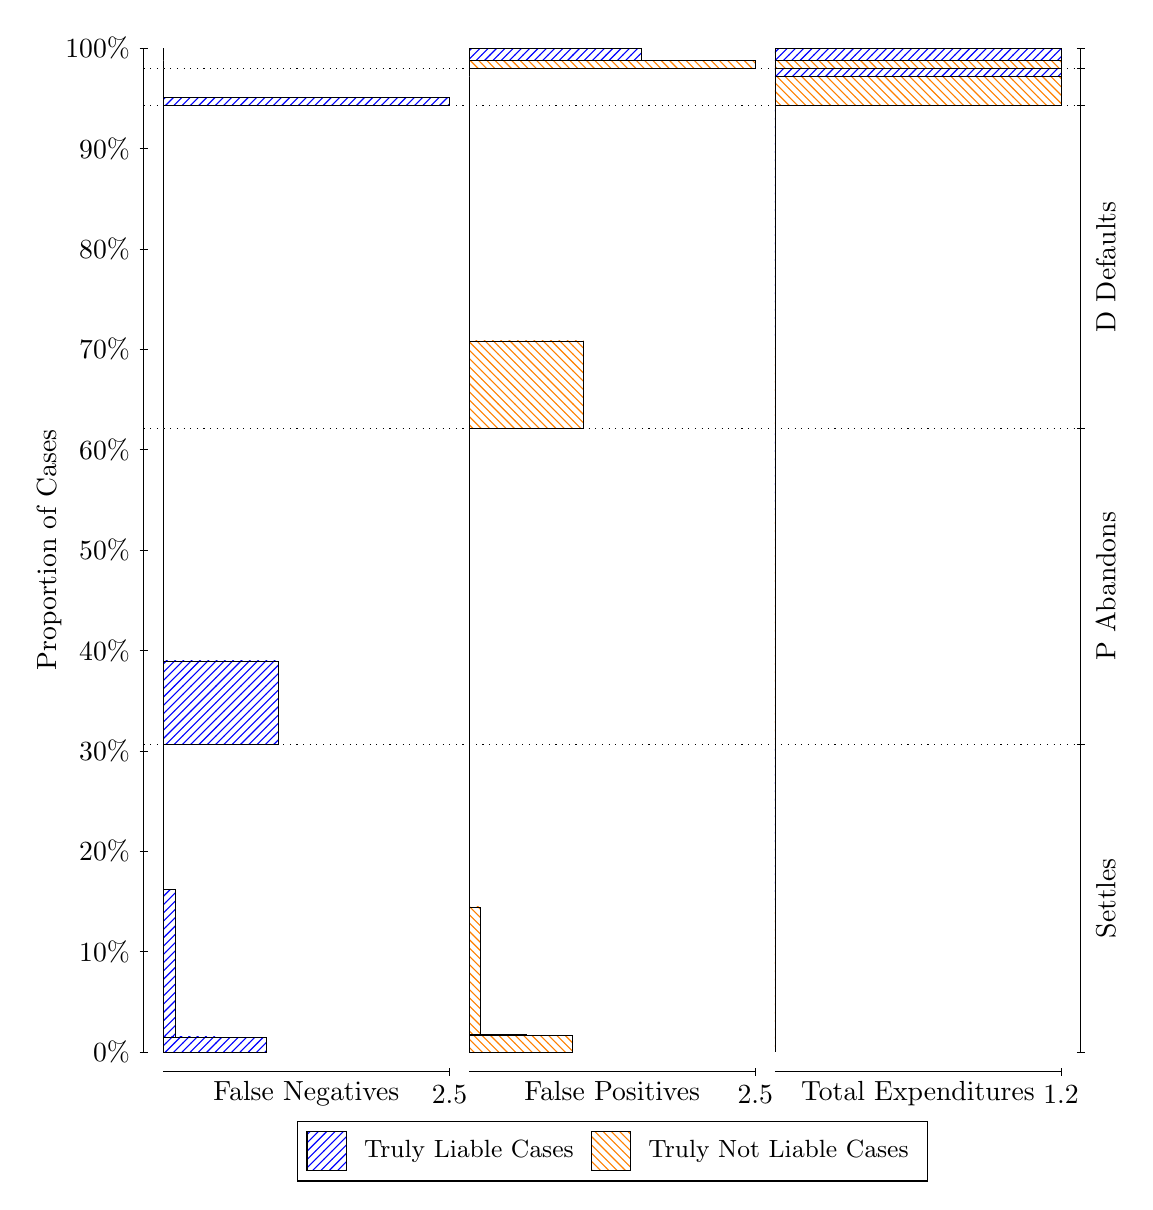
\begin{tikzpicture}
\draw[black, very thin] (1.5,1.75) -- (1.5,14.5);
\node[rotate=90, anchor=center] at (0.3, 8.125) {Proportion of Cases};
\draw[black, very thin] (1.45,1.75) -- (1.55,1.75);
\node[anchor=east] at (1.45, 1.75) {0\%};
\draw[black, very thin] (1.45,3.025) -- (1.55,3.025);
\node[anchor=east] at (1.45, 3.025) {10\%};
\draw[black, very thin] (1.45,4.3) -- (1.55,4.3);
\node[anchor=east] at (1.45, 4.3) {20\%};
\draw[black, very thin] (1.45,5.575) -- (1.55,5.575);
\node[anchor=east] at (1.45, 5.575) {30\%};
\draw[black, very thin] (1.45,6.85) -- (1.55,6.85);
\node[anchor=east] at (1.45, 6.85) {40\%};
\draw[black, very thin] (1.45,8.125) -- (1.55,8.125);
\node[anchor=east] at (1.45, 8.125) {50\%};
\draw[black, very thin] (1.45,9.4) -- (1.55,9.4);
\node[anchor=east] at (1.45, 9.4) {60\%};
\draw[black, very thin] (1.45,10.675) -- (1.55,10.675);
\node[anchor=east] at (1.45, 10.675) {70\%};
\draw[black, very thin] (1.45,11.95) -- (1.55,11.95);
\node[anchor=east] at (1.45, 11.95) {80\%};
\draw[black, very thin] (1.45,13.225) -- (1.55,13.225);
\node[anchor=east] at (1.45, 13.225) {90\%};
\draw[black, very thin] (1.45,14.5) -- (1.55,14.5);
\node[anchor=east] at (1.45, 14.5) {100\%};

\draw[black, very thin] (13.4,1.75) -- (13.4,14.5);
\draw[black, very thin] (13.35,1.75) -- (13.45,1.75);
\node[anchor=west] at (13.35, 1.75) {};
\draw[black, very thin] (13.35,5.655) -- (13.45,5.655);
\node[anchor=west] at (13.35, 5.655) {};
\draw[black, very thin] (13.35,9.6692) -- (13.45,9.6692);
\node[anchor=west] at (13.35, 9.6692) {};
\draw[black, very thin] (13.35,13.769) -- (13.45,13.769);
\node[anchor=west] at (13.35, 13.769) {};
\draw[black, very thin] (13.35,14.242) -- (13.45,14.242);
\node[anchor=west] at (13.35, 14.242) {};
\draw[black, very thin] (13.35,14.5) -- (13.45,14.5);
\node[anchor=west] at (13.35, 14.5) {};

\draw[black, very thin, pattern color=blue, pattern=north east lines] (1.75,1.75) rectangle (3.058,1.9348);
\draw[black, very thin, pattern color=blue, pattern=north east lines] (1.75,1.9348) rectangle (2.9127,1.935);
\draw[black, very thin, pattern color=blue, pattern=north east lines] (1.75,1.935) rectangle (2.7673,1.9352);
\draw[black, very thin, pattern color=blue, pattern=north east lines] (1.75,1.9352) rectangle (2.622,1.9354);
\draw[black, very thin, pattern color=blue, pattern=north east lines] (1.75,1.9354) rectangle (2.622,1.9354);
\draw[black, very thin, pattern color=blue, pattern=north east lines] (1.75,1.9354) rectangle (2.4767,1.9413);
\draw[black, very thin, pattern color=blue, pattern=north east lines] (1.75,1.9413) rectangle (2.3313,1.9417);
\draw[black, very thin, pattern color=blue, pattern=north east lines] (1.75,1.9417) rectangle (2.186,1.9422);
\draw[black, very thin, pattern color=blue, pattern=north east lines] (1.75,1.9422) rectangle (2.0407,1.9426);
\draw[black, very thin, pattern color=blue, pattern=north east lines] (1.75,1.9426) rectangle (1.8953,3.8136);
\draw[black, very thin, pattern color=orange, pattern=north west lines] (1.75,3.8136) rectangle (1.75,5.655);
\draw[black, very thin, pattern color=blue, pattern=north east lines] (1.75,5.655) rectangle (3.2033,6.7181);
\draw[black, very thin, pattern color=orange, pattern=north west lines] (1.75,6.7181) rectangle (1.75,9.6692);
\draw[black, very thin, pattern color=orange, pattern=north west lines] (1.75,9.6692) rectangle (1.75,10.78);
\draw[black, very thin, pattern color=blue, pattern=north east lines] (1.75,10.78) rectangle (1.75,13.769);
\draw[black, very thin, pattern color=blue, pattern=north east lines] (1.75,13.769) rectangle (5.3833,13.87);
\draw[black, very thin, pattern color=orange, pattern=north west lines] (1.75,13.87) rectangle (1.75,14.242);
\draw[black, very thin, pattern color=orange, pattern=north west lines] (1.75,14.242) rectangle (1.75,14.342);
\draw[black, very thin, pattern color=blue, pattern=north east lines] (1.75,14.342) rectangle (1.75,14.5);
\draw[black, very thin, pattern color=orange, pattern=north west lines] (5.6333,1.75) rectangle (6.9413,1.9637);
\draw[black, very thin, pattern color=orange, pattern=north west lines] (5.6333,1.9637) rectangle (6.796,1.9642);
\draw[black, very thin, pattern color=orange, pattern=north west lines] (5.6333,1.9642) rectangle (6.6507,1.9646);
\draw[black, very thin, pattern color=orange, pattern=north west lines] (5.6333,1.9646) rectangle (6.5053,1.965);
\draw[black, very thin, pattern color=orange, pattern=north west lines] (5.6333,1.965) rectangle (6.36,1.9709);
\draw[black, very thin, pattern color=orange, pattern=north west lines] (5.6333,1.9709) rectangle (6.2147,1.9709);
\draw[black, very thin, pattern color=orange, pattern=north west lines] (5.6333,1.9709) rectangle (6.2147,1.9711);
\draw[black, very thin, pattern color=orange, pattern=north west lines] (5.6333,1.9711) rectangle (6.0693,1.9713);
\draw[black, very thin, pattern color=orange, pattern=north west lines] (5.6333,1.9713) rectangle (5.924,1.9715);
\draw[black, very thin, pattern color=orange, pattern=north west lines] (5.6333,1.9715) rectangle (5.7787,3.5915);
\draw[black, very thin, pattern color=blue, pattern=north east lines] (5.6333,3.5915) rectangle (5.6333,5.655);
\draw[black, very thin, pattern color=orange, pattern=north west lines] (5.6333,5.655) rectangle (5.6333,8.6061);
\draw[black, very thin, pattern color=blue, pattern=north east lines] (5.6333,8.6061) rectangle (5.6333,9.6692);
\draw[black, very thin, pattern color=orange, pattern=north west lines] (5.6333,9.6692) rectangle (7.0867,10.78);
\draw[black, very thin, pattern color=blue, pattern=north east lines] (5.6333,10.78) rectangle (5.6333,13.769);
\draw[black, very thin, pattern color=orange, pattern=north west lines] (5.6333,13.769) rectangle (5.6333,14.141);
\draw[black, very thin, pattern color=blue, pattern=north east lines] (5.6333,14.141) rectangle (5.6333,14.242);
\draw[black, very thin, pattern color=orange, pattern=north west lines] (5.6333,14.242) rectangle (9.2667,14.342);
\draw[black, very thin, pattern color=blue, pattern=north east lines] (5.6333,14.342) rectangle (7.8133,14.5);
\draw[black, very thin, pattern color=orange, pattern=north west lines] (9.5167,1.75) rectangle (9.5167,3.5915);
\draw[black, very thin, pattern color=blue, pattern=north east lines] (9.5167,3.5915) rectangle (9.5167,5.655);
\draw[black, very thin, pattern color=orange, pattern=north west lines] (9.5167,5.655) rectangle (9.5167,8.6061);
\draw[black, very thin, pattern color=blue, pattern=north east lines] (9.5167,8.6061) rectangle (9.5167,9.6692);
\draw[black, very thin, pattern color=orange, pattern=north west lines] (9.5167,9.6692) rectangle (9.5167,10.78);
\draw[black, very thin, pattern color=blue, pattern=north east lines] (9.5167,10.78) rectangle (9.5167,13.769);
\draw[black, very thin, pattern color=orange, pattern=north west lines] (9.5167,13.769) rectangle (13.15,14.141);
\draw[black, very thin, pattern color=blue, pattern=north east lines] (9.5167,14.141) rectangle (13.15,14.242);
\draw[black, very thin, pattern color=orange, pattern=north west lines] (9.5167,14.242) rectangle (13.15,14.342);
\draw[black, very thin, pattern color=blue, pattern=north east lines] (9.5167,14.342) rectangle (13.15,14.5);
\draw[black, dotted] (1.5,5.655) -- (13.4,5.655);
\draw[black, dotted] (1.5,9.6692) -- (13.4,9.6692);
\draw[black, dotted] (1.5,13.769) -- (13.4,13.769);
\draw[black, dotted] (1.5,14.242) -- (13.4,14.242);
\draw[black, very thin] (1.75,1.5) -- (5.3833,1.5);
\node[anchor=north] at (3.5667, 1.5) {False Negatives};
\draw[black, very thin] (5.3833,1.45) -- (5.3833,1.55);
\node[anchor=north] at (5.3833, 1.45) {2.5};

\draw[black, very thin] (5.6333,1.5) -- (9.2667,1.5);
\node[anchor=north] at (7.45, 1.5) {False Positives};
\draw[black, very thin] (9.2667,1.45) -- (9.2667,1.55);
\node[anchor=north] at (9.2667, 1.45) {2.5};

\draw[black, very thin] (9.5167,1.5) -- (13.15,1.5);
\node[anchor=north] at (11.333, 1.5) {Total Expenditures};
\draw[black, very thin] (13.15,1.45) -- (13.15,1.55);
\node[anchor=north] at (13.15, 1.45) {1.2};

\node[black, centered, rotate=90] at (13.72, 3.7025) {Settles};
\node[black, centered, rotate=90] at (13.72, 7.6621) {P Abandons};
\node[black, centered, rotate=90] at (13.72, 11.719) {D Defaults};



\draw (7.449999999999999,1.5) node[draw=none] (baseCoordinate) {};
\begin{scope}[align=center]
        \matrix[scale=0.5, draw=black, below=0.5cm of baseCoordinate, nodes={draw}, column sep=0.1cm]{
            \node[rectangle, draw, minimum width=0.5cm, minimum height=0.5cm, pattern=north east lines, pattern color=blue] {}; &
            \node[draw=none, font=\small] (B) {Truly Liable Cases}; &
            \node[rectangle, draw, minimum width=0.5cm, minimum height=0.5cm, pattern=north west lines, pattern color=orange] {}; &
            \node[draw=none, font=\small] (B) {Truly Not Liable Cases}; \\
            };
\end{scope}

\end{tikzpicture}
\end{document}